\documentclass[sigplan,screen]{acmart}
\settopmatter{printccs=false, printacmref=false}

\setcopyright{none}
\acmPrice{}
\acmDOI{}
\acmYear{}
\copyrightyear{}
\acmISBN{}
\acmConference[FARM '22]{}
\acmBooktitle{}

%% Bibliography style
\bibliographystyle{ACM-Reference-Format}
%% Citation style
%% Note: author/year citations are required for papers published as an
%% issue of PACMPL.
\citestyle{acmauthoryear}   %% For author/year citations

%% Some recommended packages.
\usepackage{booktabs}   %% For formal tables:
                        %% http://ctan.org/pkg/booktabs
\usepackage{subcaption} %% For complex figures with subfigures/subcaptions
                        %% http://ctan.org/pkg/subcaption
\usepackage{alltt}

\begin{document}

%% Title information
\title{Demo: Counterpoint Analysis and Synthesis}
%\subtitle{Functional Pearl}

%% Author information
%% Contents and number of authors suppressed with 'anonymous'.

\author{John Leo}
\affiliation{
  \institution{Halfaya Research}
  \city{Bellevue}
  \state{WA}
  \country{USA}
}
\email{leo@halfaya.org}


%% Abstract
%% Note: \begin{abstract}...\end{abstract} environment must come
%% before \maketitle command
\begin{abstract}
We present a Haskell library to help analyze
and synthesize musical counterpoint. The tool allows expression of
generic constraints in a higher-level musical language which are
translated to a lower level for use both to find rule violations in
existing music and to generate (using an SMT solver) new
music satisfying the constraints. The tool is intended for use by
musicians who need only have a basic knowledge of Haskell.
\end{abstract}


%% 2012 ACM Computing Classification System (CSS) concepts
%% Generate at 'http://dl.acm.org/ccs/ccs.cfm'.
\begin{CCSXML}
<ccs2012>
<concept>
<concept_id>10010405.10010469.10010475</concept_id>
<concept_desc>Applied computing~Sound and music computing</concept_desc>
<concept_significance>500</concept_significance>
</concept>
<concept>
<concept_id>10011007.10011006.10011008.10011009.10011012</concept_id>
<concept_desc>Software and its engineering~Functional languages</concept_desc>
<concept_significance>500</concept_significance>
</concept>
</ccs2012>
\end{CCSXML}

\ccsdesc[500]{Applied computing~Sound and music computing}
\ccsdesc[500]{Software and its engineering~Functional languages}
%% End of generated code

%% Keywords
%% comma separated list
\keywords{Counterpoint, Haskell, SMT}  %% \keywords are mandatory in final camera-ready submission


%% \maketitle
%% Note: \maketitle command must come after title commands, author
%% commands, abstract environment, Computing Classification System
%% environment and commands, and keywords command.
\maketitle

\section{Introduction}

We demonstrate work in progress on a tool to assist in the analysis of
synthesis of musical counterpoint. Since the mid-18th century, the
composition of counterpoint has been guided by principles enunciated
in Fux's \textit{Gradus ad Parnassum} \citep{Fux1965}, first published
in 1725. Fux presents an increasingly sophisticated series of
``species'' (one note against one note, two notes against one note,
etc.) along with rules governing intervals between notes and motion
between intervals designed to ensure consonance and independence of
voices. It is well documented \citep{Mann1987} that composers
including Haydn, Mozart and Beethoven both studied and taught from
this text, and its fundamentals continue to be taught to music students
today (for example \cite{Kennan1999, Aldwell2018}).

In previous work, Cong and Leo \citep{CongLeo2019} encode the rules of
first-species (note against note) counterpoint as type constructors in
the dependently-typed language Agda. This enforces
correct-by-construction counterpoint and allows use of the Agda
typechecker to return errors with no additional effort required. On
the down side, these errors can be difficult to interpret for those
less familiar with type errors. Furthermore, encoding rules into
constructors is awkward for handling more complex species and more
global constraints. One could separate the construction of the pure
music from the constraints which can be added as a local or global
predicate (as in refinement types), but one may also wish to
deliberately violate some of the rules of strict counterpoint, as
composers often do in practice, and simply be informed of where the
violations occur without being prohibited from incorporating them.

Another approach then is to write a special-purpose ``type checker''
which can be run on previously-created music and which can generate
clear and precise error messages which are musically meaningful. The
checker is ideally easily customizable in terms of what constraints
one would like to impose. It turns out these constraints can be
expressed (at a low level) in the quantifier-free logic of linear
arithmetic and uninterpreted functions (QF-UFLIA \cite{Barrett2010}),
which allows one to not only analyze existing counterpoint, but also
synthesize counterpoint satisfying the constraints using an SMT
solver.

This tool, still a work in progress, has been implemented in Haskell
and is available at \cite{HaskellCounterpoint}. Haskell was chosen as
a high-quality and feature-rich SMT library called SBV \citep{SBV} is
available. The tool makes heavy use of functional programming, but
dependent types are sometimes wished for and the goal is to eventually
port the work to the Agda Music Tools \cite{MusicTools} library.

The following sections give an overview of current
functionality. Future plans include integration with Liquid Haskell
\citep{LiquidHaskell} (for analysis) and Synquid \citep{Synquid} (for
synthesis). In addition to handling higher species we would like to
also incorporate the rules and conventions of galant schemata
\citep{Gjerdingen2007}, which informed much of the music composed in
the era of Haydn and Mozart. Ideally one could use the tool to compose
convincing music in the galant style.

Concurrently Cong \citep{Cong2022a} is exploring another approach
using a different representation of constraints within a type system.

\section{An Example}

We briefly describe one way in which this tool can be used for both
analysis and synthesis. We first examine the example numbered 146 in
the critical edition of Beethoven's studies with Haydn
(\cite{BeethovenWerke13}; see also \cite{Nottebohm1971}, p.\ 31 and
\cite{Mann1987}, p.\ 115). It is shown in modern notation in
Figure~\ref{fig:b146}.

\begin{figure}
  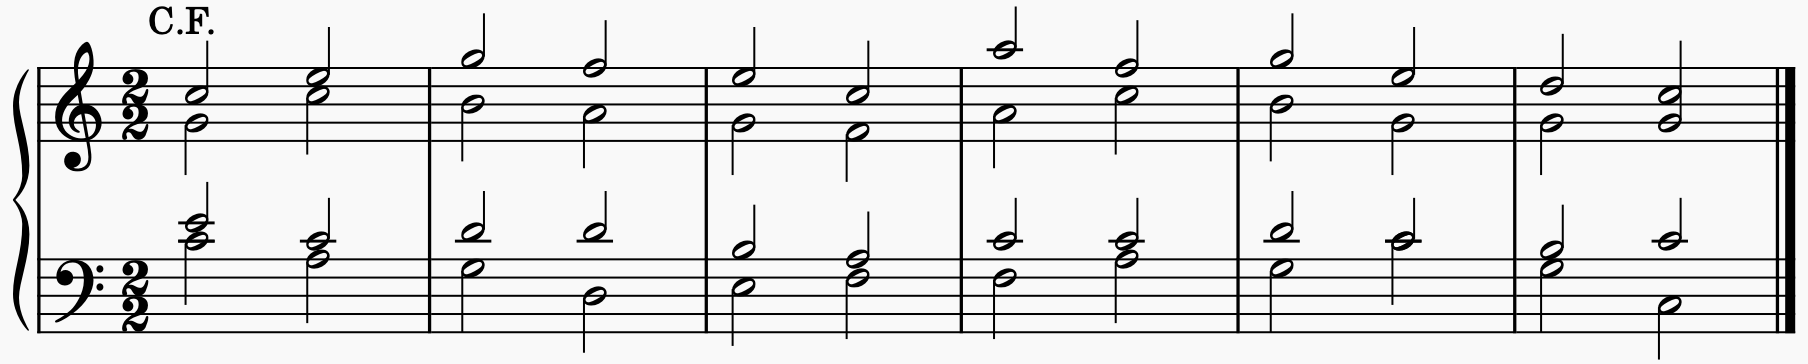
\includegraphics[width=8cm]{figures/b146.png}
  \caption{Beethoven Exercise 146}
  \Description{Beethoven Exercise 146}
  \label{fig:b146}
\end{figure}

Here Haydn has supplied the top voice, marked ``C.F.'' for cantus
firmus, and Beethoven's task was to supply the remaining three voices
following first species counterpoint rules. He uses only tones from
triads, all of them complete save the last and all in root position
save the second triad in bar 4. Since the notes form triads they
automatically satisfy consonance rules (only perfect intervals, thirds
or sixths between any pair of notes vertically); note that a perfect
fourth is prohibited in two part strict counterpoint but allowed with
more voices. Perfect fourths can be found between the top two voices
in the first, fourth and last bars.

There are boundary rules that the top and bottom voices must form
octaves at the beginning and end, and motion rules which are designed
to ensure independence of voices. In particular parallel and similar
(both voices moving in the same direction) motion into fifths and
octaves is prohibited. Here we can see that Beethoven has in fact made
two errors in the top two voices: similar motion into a fifth in bar 3
and then into an octave between bars 3 and 4. Haydn fixes both errors
by changing the F in the second voice to an A.

For simplicity we now focus only on the top two voices. Feeding
Beethoven's notes into the tool as two part first species
counterpoint, it easily finds and reports errors in the use of perfect
fourths, missing octaves at the boundaries, and similar motion into
fifths and octaves. We can disable the boundary rules as they are not
relevant and relax the consonance rule to allow perfect fourths, leaving
only the motion errors. We can replace the note F that Haydn fixed
with a hole, and run the tool in synthesis mode using the same
rules. It makes the same fix Haydn did. Perhaps we gave it too much
guidance, so instead we can create three holes in a row near the
error, which generates the solution shown in
Figure~\ref{fig:b146fix3}. Note that this introduces a series of five
parallel 6ths, and there is a ``soft'' rule that one should not have
long sequences of 3rds or 6ths as that also diminishes independence
of voices. However we can easily add a constraint limiting parallel
intervals to at most two in a row; the solution returned changes the G
in bar three to an A, breaking the chain with a fifth, a small
improvement but one might hope for more.

\begin{figure}
  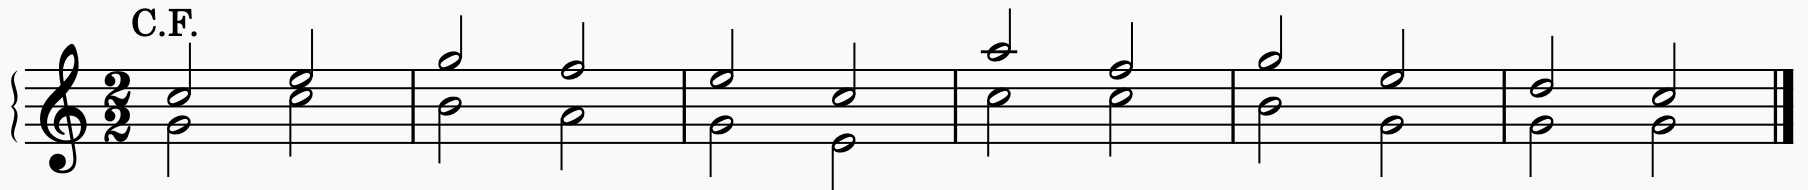
\includegraphics[width=8cm]{figures/b146fix3.png}
  \caption{Three Notes Changed}
  \Description{Three Notes Changed}
  \label{fig:b146fix3}
\end{figure}

This can be done by adding a constraint to increase contrary motion
(in which both voices move in opposite directions), and in fact we can
try generating our own two part counterpoint following Haydn's cantus
firmus, fixing only the first and last of Beethoven's notes. To help
create better quality counterpoint we add constraints to limit the
number of leaps (horizontal intervals of more than a major third) to
at most one and require at least six instances of contrary motion,
which turns out to be maximal. Note that it would be extremely
difficult for a human being with no computer assistance to generate
counterpoint following such restrictions, but the SMT solver instantly
returns the solution shown in Figure~\ref{fig:b146gen3}.

\begin{figure}
  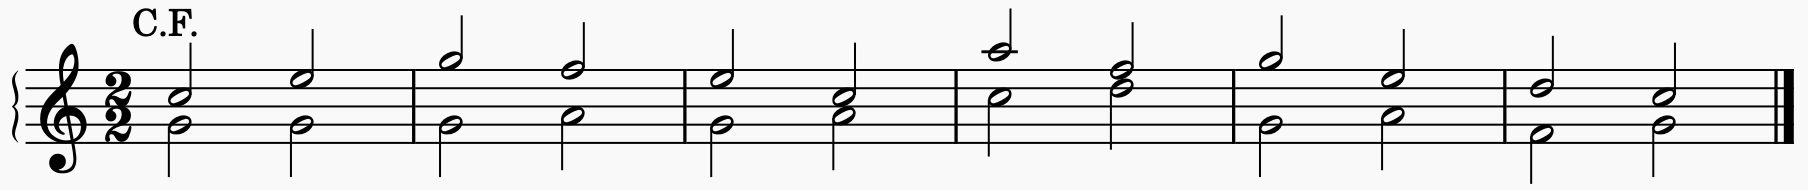
\includegraphics[width=8cm]{figures/b146gen3.png}
  \caption{Generated Counterpoint}
  \Description{Generated Counterpoint}
  \label{fig:b146gen3}
\end{figure}


\section{Selected Features}

We describe at a high level some of the key features of the
library. Details can be found in the code repository
\citep{HaskellCounterpoint}.

At a high level music is represented as a list of voices, which in
turn are a list of bars, which are in turn a list of beats. Here
dependent types would be useful to ensure for example that every voice
has the same number of bars, but a run-time check can also be used to
enforce this. Each of these elements is parameterized, allowing a
number of pitch-like elements to be used to construct music. These
could be algebraic data types representing name (like C\#) and
octave, or a numeric representation of pitch. Either datum can then be
embedded into a wrapper, such as \texttt{MPitch} which can either be a
fixed pitch or a named hole to be solved for.

The above representation of music allows natural handling of first,
second and third species counterpoint (one to four notes per cantus
firmus note) as well as multi-part counterpoint. At a lower level the
music is translated into a simpler form---for example first-species
two part counterpoint is most simply represented as a list of pairs.

We plan to try to implement a constraint language as an embedded
DSL. However for now Haskell typeclasses are used, which have the
advantage that constraints can be written in natural Haskell; the only
drawback is that type signatures are somewhat abstract. The main
challenge is that we want to write constraints only once and use them
for both analysis and synthesis. The former expects low-level integers
and booleans while the latter their symbolic counterparts. This is
handled by using typeclasses which can be instantiated with either.

Analysis and synthesis then both take the same music and list of
constraints. The former checks the constraints returning error
messages in the higher-level language used to express the music. The
latter generates (if possible) music by filling in the given holes
using the constraints and the SMT solver. MIDI is also generated,
which can then be opened and viewed with notation software such as
MuseScore.

\section*{Acknowledgements}

Thanks to Youyou Cong for many enlightening discussions about type
theory and music over the past several years, and for suggesting to
look at Beethoven's exercises as a source of examples. Thanks also to
Emina Torlak and Stephen Rumph for their generosity in allowing me to
audit their classes at the University of Washington. CSE 507 was
invaluable for learning the fundamentals of SMT 
solvers, and MUHST 211 and 430 introduced me to galant schemata.

%% Bibliography
\bibliography{abstract.bib}

\end{document}
